%%%%%%%%%%%%%%%%%%%%%%%%%%%%%%%%%%%%%%%%%
% Jacobs Landscape Poster
% LaTeX Template
% Version 1.1 (14/06/14)
%
% Created by:
% Computational Physics and Biophysics Group, Jacobs University
% https://teamwork.jacobs-university.de:8443/confluence/display/CoPandBiG/LaTeX+Poster
% 
% Further modified by:
% Nathaniel Johnston (nathaniel@njohnston.ca)
%
% This template has been downloaded from:
% http://www.LaTeXTemplates.com
%
% License:
% CC BY-NC-SA 3.0 (http://creativecommons.org/licenses/by-nc-sa/3.0/)
%
%%%%%%%%%%%%%%%%%%%%%%%%%%%%%%%%%%%%%%%%%

%----------------------------------------------------------------------------------------
%	PACKAGES AND OTHER DOCUMENT CONFIGURATIONS
%----------------------------------------------------------------------------------------

\documentclass[final]{beamer}

\usepackage[scale=1.0]{beamerposter} % Use the beamerposter package for laying out the poster
\usetheme{confposter} % Use the confposter theme supplied with this template

\setbeamercolor{block title}{fg=dblue!80,bg=white} % Colors of the block titles
\setbeamercolor{block body}{fg=black,bg=white} % Colors of the body of blocks
\setbeamercolor{block alerted title}{fg=white,bg=dblue!70} % Colors of the highlighted block titles
\setbeamercolor{block alerted body}{fg=black,bg=dblue!10} % Colors of the body of highlighted blocks
% Many more colors are available for use in beamerthemeconfposter.sty

%-----------------------------------------------------------
% Define the column widths and overall poster size
% To set effective sepwid, onecolwid and twocolwid values, first choose how many columns you want and how much separation you want between columns
% In this template, the separation width chosen is 0.024 of the paper width and a 4-column layout
% onecolwid should therefore be (1-(# of columns+1)*sepwid)/# of columns e.g. (1-(4+1)*0.024)/4 = 0.22
% onecolwid should therefore be (1-(# of columns+1)*sepwid)/# of columns e.g. 
% (1-(3+1)*0.025)/3 = 0.3
% Set twocolwid to be (2*onecolwid)+sepwid = 0.464
% Set threecolwid to be (3*onecolwid)+2*sepwid = 0.708

\newlength{\sepwid}
\newlength{\onecolwid}
\newlength{\twocolwid}
\newlength{\threecolwid}
\setlength{\paperwidth}{36in} % A0 width: 46.8in
\setlength{\paperheight}{48in} % A0 height: 33.1in
\setlength{\textwidth}{34in} % A0 width: 46.8in
\setlength{\textheight}{46in} % A0 height: 33.1in
\setlength{\sepwid}{0.025\paperwidth} % Separation width (white space) between columns
\setlength{\onecolwid}{0.3\paperwidth} % Width of one column
\setlength{\twocolwid}{0.625\paperwidth} % Width of two columns
\setlength{\threecolwid}{0.95\paperwidth} % Width of three columns
\setlength{\topmargin}{-0.5in} % Reduce the top margin size
%-----------------------------------------------------------

\usepackage{graphicx}  % Required for including images
\newcommand{\Cyclus}{\textsc{Cyclus}\xspace}%

\usepackage{tabularx}
\newcolumntype{b}{X}
\newcolumntype{s}{>{\hsize=.5\hsize}X}
\newcolumntype{m}{>{\hsize=.75\hsize}X}
\newcolumntype{z}{>{\hsize=.65\hsize}X}

\usepackage{booktabs} % Top and bottom rules for tables
\usepackage{xspace}

\usepackage{tikz}
\usetikzlibrary{positioning, arrows, decorations, shapes, arrows.meta}
% Define block styles
\tikzstyle{decision} = [diamond, draw, fill=blue!20, 
text width=4.5em, text badly centered, node distance=3cm, inner sep=0pt]


\tikzstyle{block} = [rectangle, draw, text centered, fill=blue!20]
\tikzstyle{line} = [draw, -latex']
\tikzstyle{cloud} = [draw, ellipse,fill=red!20, node distance=6em,
minimum height=2em]



\usetikzlibrary{shapes.multipart}
\usetikzlibrary{positioning}


\setbeamertemplate{bibliography item}[text]

%----------------------------------------------------------------------------------------
%	TITLE SECTION 
%----------------------------------------------------------------------------------------

\title{
	
\includegraphics[width=0.3\linewidth]{UIUC_Logo}
	\hspace{30cm}
	\vspace{2cm}
	
\includegraphics[width=0.3\linewidth]{cnec_logo.png} \\
	Signatures and Observables of the Nuclear Fuel Cycle
} % Poster title

\author{\textbf{Gregory T. Westphal}, Kathryn D. Huff}
\institute{University of Illinios at Urbana-Champaign, Department of Nuclear, Plasma, and Radiological Engineering, Urbana, IL 61801}
%----------------------------------------------------------------------------------------

\begin{document}

\addtobeamertemplate{block end}{}{\vspace*{2ex}} % White space under blocks
\addtobeamertemplate{block alerted end}{}{\vspace*{2ex}} % White space under highlighted (alert) blocks

\setlength{\belowcaptionskip}{2ex} % White space under figures
\setlength\belowdisplayshortskip{2ex} % White space under equations

\begin{frame}[t] % The whole poster is enclosed in one beamer frame

\begin{columns}[t,totalwidth=\threecolwid] % The whole poster consists of three major columns, the second of which is split into two columns twice - the [t] option aligns each column's content to the top

\begin{column}{0.5\sepwid}\end{column} % Empty spacer column

\begin{column}{\onecolwid} % The first column

%----------------------------------------------------------------------------------------
%	OBJECTIVES
%----------------------------------------------------------------------------------------

\begin{alertblock}{Objectives}
\begin{itemize}
        \item Create high-fidelity reprocessing facility agent models (both 
                aqueous and electrochemical/pyroprocessing).
        \item Apply these models in Cyclus to simulate material diversion in closed 
                fuel cycles. 
	\item Identify and characterize non-traditional signatures and 
                observables in these facilities.
	\item Extend successful algorithms for modeling diversion and diversion 
                detection.
        \item Characterize required detection sensitivities and corresponding 
                false positive rates. 
\end{itemize}

\end{alertblock}

%----------------------------------------------------------------------------------------
%	BACKGROUND
%----------------------------------------------------------------------------------------

\begin{block}{Background}

\begin{figure}
	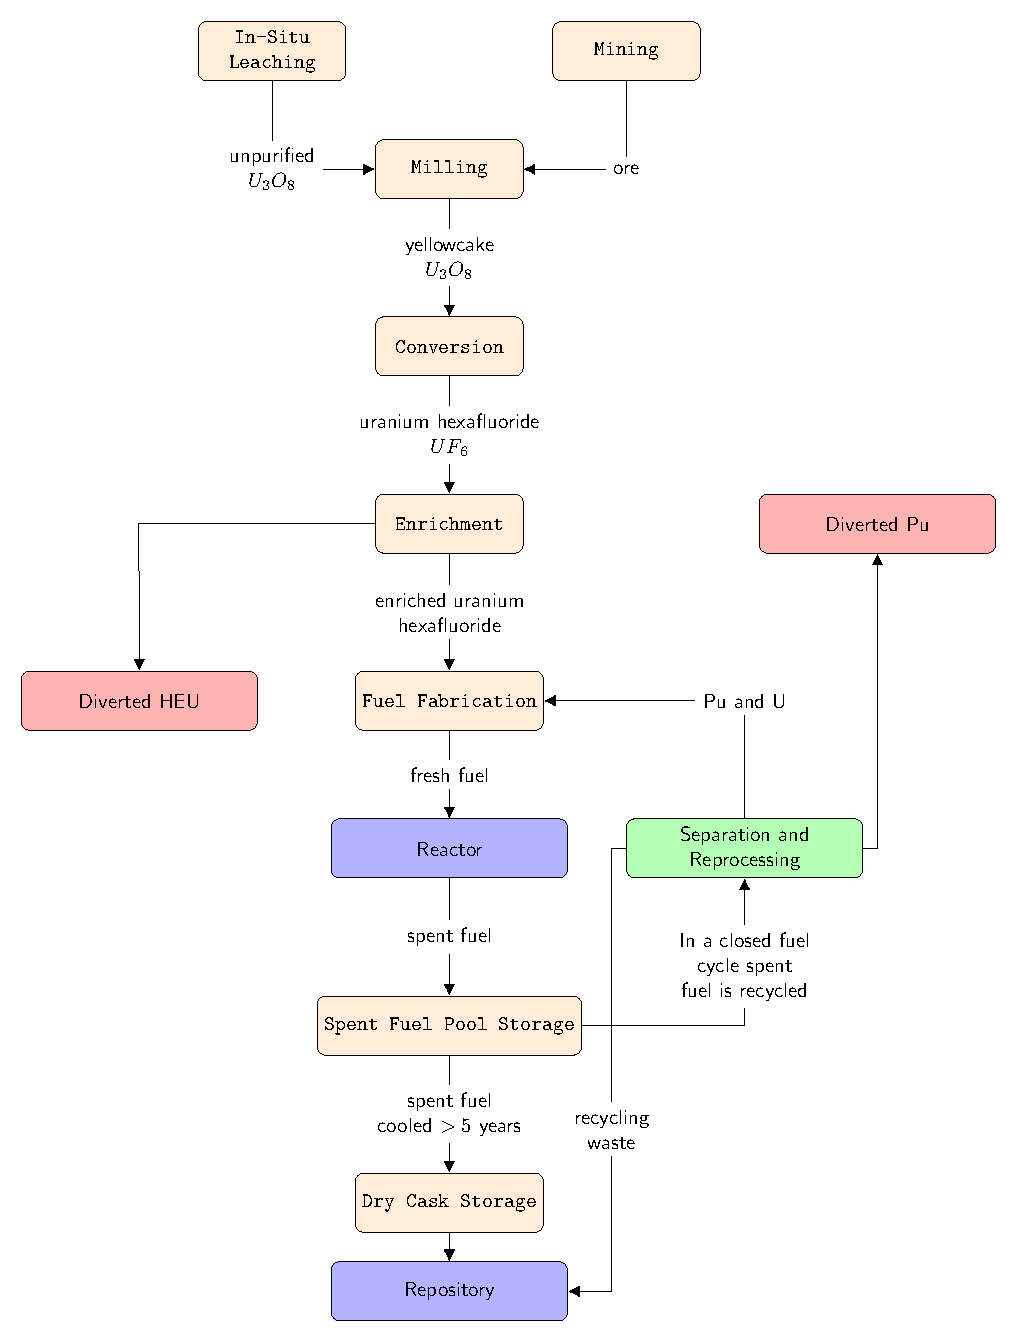
\includegraphics[width=0.75\linewidth]{fc-diagram.pdf}
%	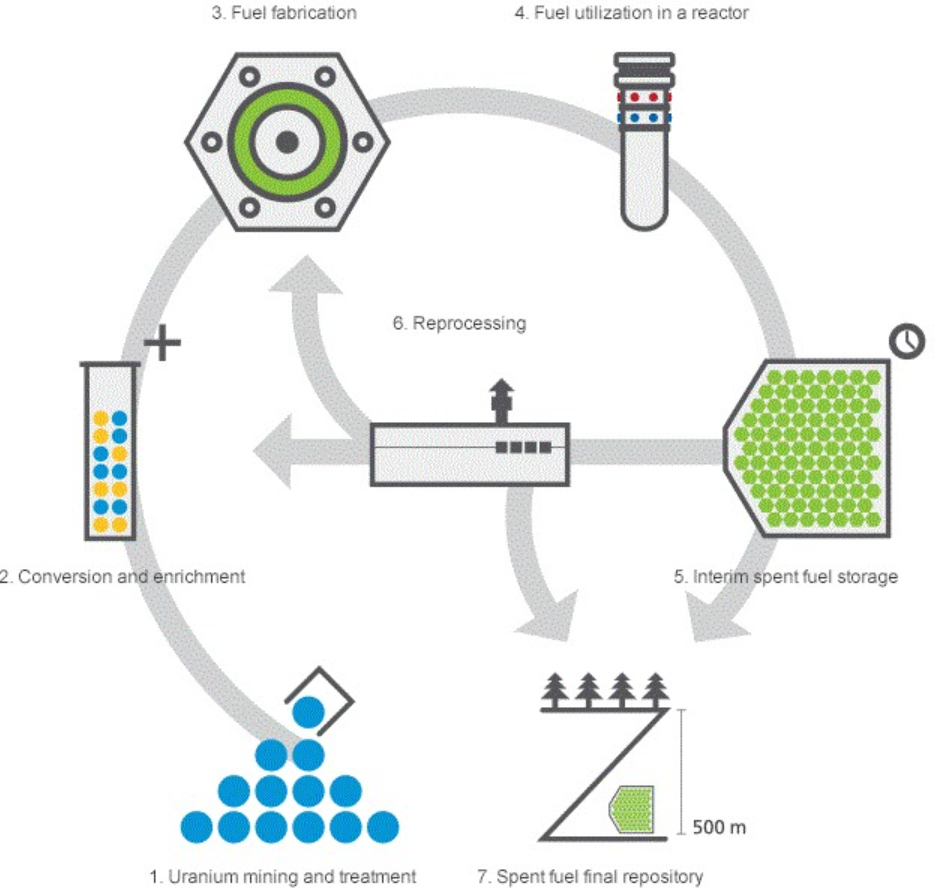
\includegraphics[width=1.0\linewidth]{fuel_cycle2.png}
        %% Diagram of the nuclear fuel cycle
% Author: Kathryn Huff
\documentclass[border=10pt]{standalone}
\usepackage{tikz}
\usetikzlibrary{arrows.meta}
\tikzset{%
  >={Latex[width=2mm,length=2mm]},
  % Specifications for style of nodes:
            base/.style = {rectangle, rounded corners, draw=black,
                           minimum width=4cm, minimum height=1cm,
                           text centered, font=\sffamily},
       bluebox/.style = {base, fill=blue!30},
       redbox/.style = {base, fill=red!30},
       greenbox/.style = {base, fill=green!30},
       process/.style = {base, minimum width=2.5cm, fill=orange!15,
                           font=\ttfamily},
}
% Drawing part, node distance is 1.5 cm and every node
% is prefilled with white background
\begin{document}
\begin{tikzpicture}[node distance=3cm,
    every node/.style={fill=white, font=\sffamily}, align=center]
  % Specification of nodes (position, etc.)
  \node (top) {};
  \node (leach)             [process, left of=top] {In-Situ\\Leaching};
  \node (mine)             [process, right of=top] {Mining};
  \node (mill)     [process, below of=top, yshift=1cm]          {Milling};
  \node (conv)      [process, below of=mill]   {Conversion};
  \node (enr)     [process, below of=conv]   {Enrichment};
  \node (fuelfab)          [process, below of=enr] {Fuel Fabrication};
  \node (reactor)      [bluebox, below of=fuelfab, yshift=0.5cm] {Reactor};
  \node (pool)       [process, below of=reactor] {Spent Fuel Pool Storage};
  \node (cask)    [process, below of=pool] {Dry Cask Storage};
  \node (reprocess)    [greenbox, right of=reactor, xshift=2cm] {Separation and\\Reprocessing};
  \node (repository) [bluebox, below of=cask, yshift=1.5cm] {Repository}; 
  \node (pdivert)    [redbox, right of=enr, xshift=4.25cm] {Diverted Pu};
  \node (heudivert)  [redbox, left of=fuelfab, xshift=-2.25cm] {Diverted HEU};
  % Specification of lines between nodes specified above
  % with aditional nodes for description 
\draw[->]     (leach) |- (mill) node[midway] {unpurified\\$U_3O_8$};
\draw[->]     (mine) |- (mill) node[midway] {ore};
\draw[->]     (mill) -- (conv) node[midway] {yellowcake\\$U_3O_8$};
\draw[->]      (conv) -- (enr) node[midway] {uranium hexafluoride\\$UF_6$};
\draw[->]     (enr) -- (fuelfab) node[midway] {enriched uranium\\hexafluoride};
  \draw[->]      (fuelfab) -- node[midway] {fresh fuel} (reactor);
  \draw[->]      (reactor) -- node[midway] {spent fuel} (pool);%\\uranium and\\fission products} (pool);
   \draw[->]       (pool) -- node[midway] {spent fuel\\cooled $>5$ years} (cask);
  \draw[->]       (pool) -| node[yshift=1cm, text width=3cm] {In a closed 
                            fuel cycle spent fuel is recycled} (reprocess);
  \draw[->]    (cask) -- (repository);
  \draw [->] (reprocess.west) -- ++(-0.25,0) -- node[yshift=-1cm] 
  {recycling\\waste} ++ (0,-7.5) -- (repository.0);
  \draw [->] (reprocess.north) |- node[midway] {Pu and U}  (fuelfab.east);
  \draw [->] (reprocess.east) -- ++(0.25,0) -- ++(0,5) (pdivert.south);
  \draw [->] (enr.west) -- ++(-4,0) -- (heudivert.north);
  %\draw[->] (reactor.east) -- ++(2.6,0) -- ++(0,2) -- ++(0,2) --                
  %   node[xshift=1.2cm,yshift=-1.5cm, text width=2.5cm]
  %   {The activity comes to the foreground}(fuelfab.east);
  \end{tikzpicture}
\end{document}


	\caption{Typical Nuclear fuel cycle without diversion \cite{huff_2018}.}
\end{figure}

\end{block}

%----------------------------------------------------------------------------------------
%	Cyclus
%----------------------------------------------------------------------------------------

\begin{block}{Cyclus}

\begin{figure}
	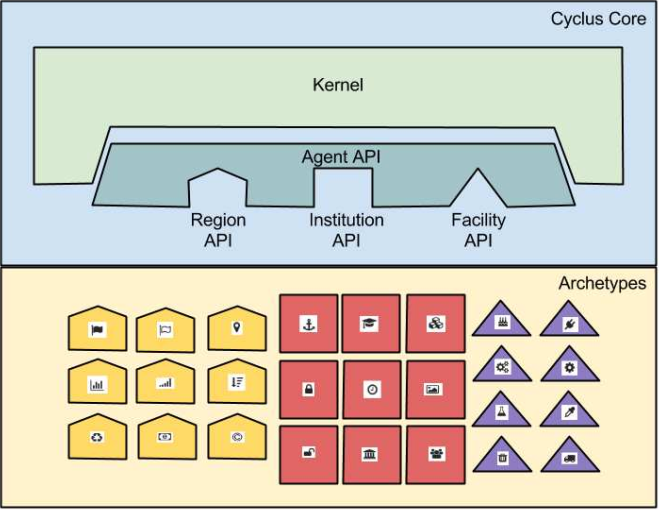
\includegraphics[width=0.9\linewidth]{Cyclus_graph}
	\caption{Cyclus API allows for modular build of simulations \cite{huff_2018}}
\end{figure}

\end{block}
%----------------------------------------------------------------------------------------

\end{column} % End of the first column

\begin{column}{\sepwid}\end{column} % Empty spacer column


%----------------------------------------------------------------------------------------

\begin{column}{\onecolwid} % The second column
%----------------------------------------------------------------------------------------
%	SIGNATURES AND OBSERVABLES
%----------------------------------------------------------------------------------------

\begin{block}{Signatures and Observables}
        Detection modes vary between each facility type, requiring a specific 
        analysis of each processing plant to determine effective signatures and 
        observables. For example, \textbf{pyroprocessing} has four major 
        systems with observable waste: electroreduction, electrorefining, electrowinning, and metal fuel fabrication\cite{Borrelli_2017}.
        These systems have the corresponding signatures:
        
\begin{block}{Direct}	
	\begin{itemize}
		\item \textbf{Metal Waste:} Solid, insoluble metal fission products.
		\item \textbf{Ceramic Waste Electrowinning:} Waste salt LiCl-KCl contains trace amounts of $^{135}$Cs and $^{137}$Cs from
		electrowinning the fuel.
		\item \textbf{Vitrified Waste:} LiCl-KCl salt that contains TRU and Sr alongside rare-earth elements precipitated into gases
		and vitrified with borosilicate glass.
		\item \textbf{Ceramic Waste Electroreduction:} Through electroreduction, Li$_2$CO$_3$ is used to separate $^{135}$Cs, $^{137}$Cs, 
		$^{129}$I and $^{14}$C which are solidified into ceramic waste.
	\end{itemize}
\end{block}
\begin{block}{Indirect}		
	\begin{itemize}
		\item \textbf{Power Draw:} Sign of overusing centrifuges \cite{Yilmaz_2016,Hou_2016}.
		\item \textbf{Smoke Production:} Reactor producing high power than rated or reported for possible
		nefarious reasons \cite{Yilmaz_2016}.
		\item \textbf{Decay Heat:} Lower decay heat in casks signifies over-reporting of waste \cite{Kemp_2016}.
		\item \textbf{Trace Quantities:} $^{135}$Xe and $^{85}$Kr are commonly emitted through processing along with tritium
		from reactors. Need sensitive equipment but difficult to hide \cite{Borrelli_2017,Kemp_2016}.
	\end{itemize}
\end{block}
\end{block}

    
%----------------------------------------------------------------------------------------
%	PREVIOUS WORK
%----------------------------------------------------------------------------------------

\begin{block}{Archetype Design}

\begin{figure}
	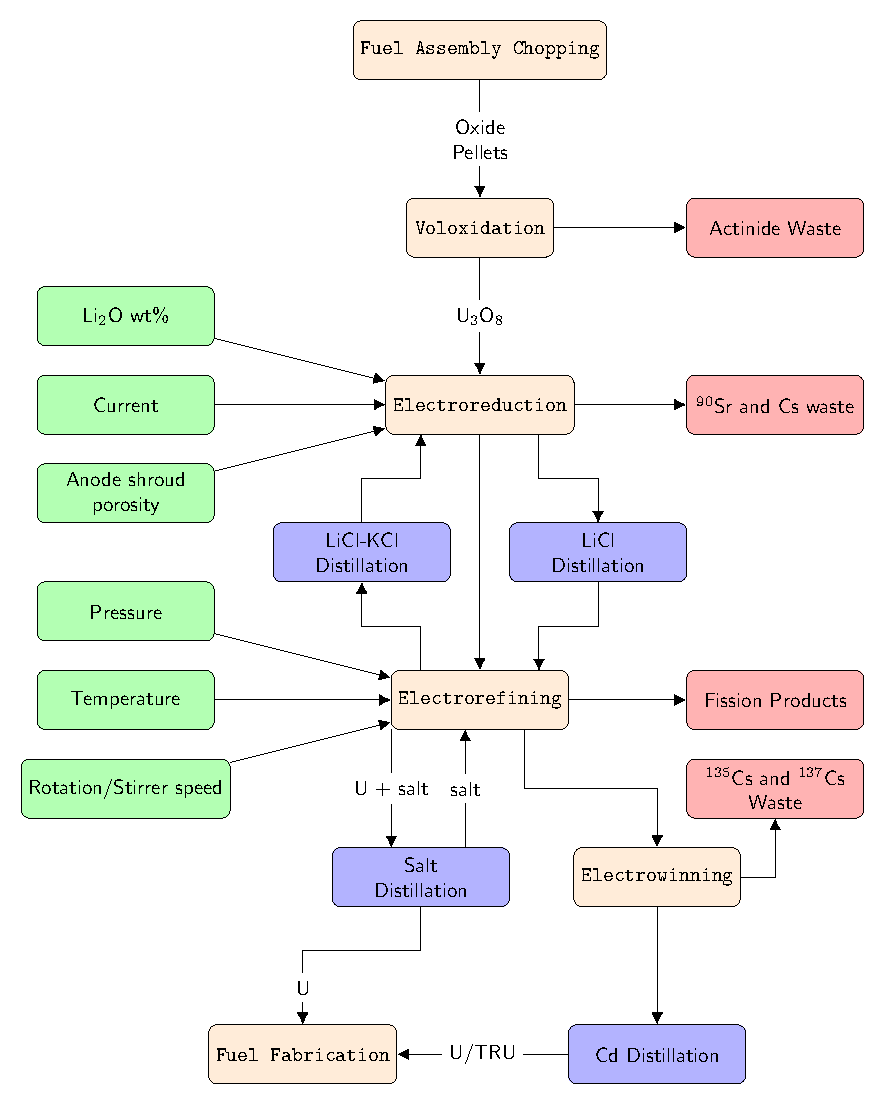
\includegraphics[width=1\linewidth]{flowchart}
	\caption{Pyroprocessing material flowchart designed for a \Cyclus archetype.}
\end{figure}

\end{block}

%----------------------------------------------------------------------------------------

\end{column} % End of column 2

\begin{column}{\sepwid}\end{column} % Empty spacer column

\begin{column}{\onecolwid} % The third column
	
%----------------------------------------------------------------------------------------
%	FUTURE WORK
%----------------------------------------------------------------------------------------

\begin{alertblock}{Future Work}
	The goal of this poster is to outline the ground work done and review previous material on diversion, particularly related
	to pyroprocessing. What needs to be accomplished proceeding this work is as follows:
	\begin{itemize}
		\item Simulate pyroprocessing plant and network.
		\item Create Cyclus output and compare to prior algorithms.
		\item Assess capability of using Cyclus as online detection.
	\end{itemize} 

\end{alertblock}


%--------------------------------------------------------
% PROJECT TIMELINE
%---------------------------------------------------------
\begin{block}{Timeline}
        \newcommand\ytl[2]{\parbox[b]{0.3\textwidth}{\hfill{\color{orange!90}\bfseries\sffamily #1}~$\cdots\cdots$~}\makebox[0pt][c]{$\bullet$}\vrule\quad 
\parbox[c]{0.7\textwidth}{\vspace{7pt}\color{dblue!80}\raggedright\sffamily #2\\[7pt]}\\[-3pt]}
\begin{table}
\centering
\begin{minipage}[t]{\linewidth}
\color{gray}
\rule{\linewidth}{1pt}
\ytl{Jan.~2018}{Project start: \hfill Literature Review.}
\ytl{Feb.~2018}{Model development: \hfill Pyro Separations}
\ytl{Mar.~2018}{Data collection: \hfill Pyro Separations}
\ytl{May.~2018}{Model development: \hfill Cyclus Pyroprocess}
\ytl{Jun.~2018}{Model development: \hfill Build Archetype}
\ytl{Jul.~2018}{Model development: \hfill Signatures Class}
\ytl{Aug.~2018}{Data collection: \hfill Cyclus Simulation}
\ytl{Sep.~2018}{Scenario simulation: \hfill Prior Observables}
\ytl{Oct.~2018}{Scenario simulation: \hfill Proposed Observables}
\ytl{Dec.~2018}{Scenario simulation: \hfill Vary algorithm}
%\ytl{~~~~~}{~~~~}
\rule{\linewidth}{1pt}%
\\%
\bigskip
\ytl{~~~~~2019}{Sensitivity analysis: \hfill Vary key parameters.}
\bigskip
\rule{\linewidth}{1pt}%
\end{minipage}%
\end{table}

\end{block}



%----------------------------------------------------------------------------------------
%	ACKNOWLEDGEMENTS
%----------------------------------------------------------------------------------------

\setbeamercolor{block title}{fg=norange,bg=white} % Change the block title color

\begin{block}{Acknowledgements}
	
	This research was performed using funding received
	from the Consortium for Nonproliferation Enabling
	Capabilities under award number 1-483313-973000-191100.
	
	\vspace{10mm}
	\begin{center}
		\begin{tabular}{ccc}
			
\includegraphics[width=0.3\linewidth]{logo.png} & 
\includegraphics[width=0.3\linewidth]{cnec_oldlogo.png}
			& 
\includegraphics[width=0.15\linewidth]{cyclus.png}
		\end{tabular}
	\end{center}
	
	
\end{block}

%----------------------------------------------------------------------------------------
%	CONTACT INFORMATION
%----------------------------------------------------------------------------------------

\setbeamercolor{block alerted title}{fg=black,bg=norange} % Change the alert block title colors
\setbeamercolor{block alerted body}{fg=black,bg=white} % Change the alert block body colors



\begin{alertblock}{Contact Information}
	\setbeamercolor{block title}{fg=norange,bg=white} % Change the block title color
	\begin{itemize}
		
		\item Web: \href{arfc.github.io}{arfc.github.io}
		\item Email: \href{mailto:gtw2@illinois.edu}{gtw2@illinois.edu}
		\item Phone: +1 (636) 284-9691
	\end{itemize}
	
\end{alertblock}

\begin{block}{References}

        {\footnotesize\bibliographystyle{abbrv} 
        \bibliography{poster}}
\end{block}


%----------------------------------------------------------------------------------------



\end{column} % End of the third column

\end{columns} % End of all the columns in the poster

\end{frame} % End of the enclosing frame

\end{document}
\begin{column}{\sepwid}\end{column} % Empty spacer column
